% ═══════════════════════════════════════════════════════════════════════
% ICAIF 2026: 7th ACM International Conference on AI in Finance
% Milan, Nov 14-17, 2026 | Extended deadline: Aug 9, 2026 AoE
% ACM sigconf, double-blind, 8 pages TOTAL (incl. figures + references)
% ═══════════════════════════════════════════════════════════════════════
\documentclass[sigconf,anonymous]{acmart}

% ── Additional packages ───────────────────────────────────────────────
\usepackage{microtype}
\usepackage{multirow}
\usepackage{enumitem}
\usepackage{amsmath}
\usepackage{xurl}
\usepackage{tikz}
\usetikzlibrary{arrows.meta,positioning,calc}
\usepackage{algorithm}
\usepackage{algorithmic}
\emergencystretch=2em

% Suppress checkpoint notes; access dates rendered via lastaccessed bib field
\def\shownote#1{\unskip\ignorespaces}

% ── Conference metadata ───────────────────────────────────────────────
\acmConference[ICAIF '26]{7th ACM International Conference on AI in Finance}{November 14--17, 2026}{Milan, Italy}
\acmYear{2026}
\setcopyright{none}
\acmISBN{}
\acmDOI{}

% ── CCS concepts ──────────────────────────────────────────────────────
\begin{CCSXML}
<ccs2012>
  <concept>
    <concept_id>10002951.10003317.10003347.10003356</concept_id>
    <concept_desc>Information systems~Retrieval models and ranking</concept_desc>
    <concept_significance>500</concept_significance>
  </concept>
  <concept>
    <concept_id>10010405.10010489</concept_id>
    <concept_desc>Applied computing~Economics</concept_desc>
    <concept_significance>300</concept_significance>
  </concept>
</ccs2012>
\end{CCSXML}

\ccsdesc[500]{Information systems~Retrieval models and ranking}
\ccsdesc[300]{Applied computing~Economics}

% ── Keywords ──────────────────────────────────────────────────────────
\keywords{financial embeddings, return correlations, peer retrieval, multimodal retrieval, financial benchmark construction}

% ── Title ─────────────────────────────────────────────────────────────
\title{Retrieving Behavioral Equity Peers from Filing Text and Return History}

% ── Authors (hidden by anonymous option) ──────────────────────────────
\author{Anonymous}
\affiliation{\institution{Anonymous Institution}}
\email{anonymous@example.com}

% ══════════════════════════════════════════════════════════════════════
\begin{document}

% ── Abstract ──────────────────────────────────────────────────────────
\begin{abstract}
We study quarterly behavioral equity-peer retrieval.  Given a focal company,
we rank five firms expected to co-move with it during the following quarter.
Co-movement is measured after removing Fama--French five-factor (FF5) exposures.
We test whether annual Form~10-K Item~1 business text available before ranking
adds information beyond recent return co-movement, and whether any gain changes
with additional return history.  Our training-free baseline uses the standardized
residual-return time series itself as each security's embedding.  Pairwise cosine
similarity over shared dates exactly equals sample residual correlation.

Six walk-forward tests use one quarter to rank firms and the next to evaluate them,
with 1,614--1,631 securities per test.  The return path attains mean normalized
discounted cumulative gain at five (NDCG@5) of $0.336$, compared with $0.300$
for term-frequency--inverse-document-frequency (TF-IDF) and $0.279$ for the
dense Granite-r2 text encoder.  Filing similarity and residual co-movement are
nearly unrelated at the pairwise level: across 1,301,691 pairs, four dense
filing encoders have Spearman correlations of only $0.029$--$0.046$ in the same
quarter and $0.027$--$0.049$ in the next.  Even so, an
80/20 combination of return- and text-based ranks, fixed after selection on
twelve earlier tests, reaches $0.373$ and
improves on the return path in all six.  With four quarters of return history, text no longer improves the
ranking.  Across 19
transitions spanning 2020--2026, the return path leads TF-IDF in 18.

For the availability audit, each five-name list is fixed before following-quarter
returns are known; missing candidates are not replaced.  Of cases with the
required inputs at ranking time, 99.2--99.6\% remain evaluable.  In this
setting, filing text offers limited help in generating candidates.  The
experiment does not test valuation-peer selection, hedge construction, trading,
or analyst outcomes, and it still requires recent return history.
\end{abstract}

\maketitle

% ══════════════════════════════════════════════════════════════════════
\section{Introduction}
\label{sec:intro}

We study \emph{behavioral equity-peer retrieval}: for a focal company, rank firms
expected to co-move with it in the next quarter after both firms' returns have
been adjusted for the Fama--French five-factor model (FF5).  We call the returns
left after this regression \emph{residual returns} and their correlation
\emph{behavioral similarity}.  One use is to generate candidates for an
equity-risk analyst investigating shared shocks not captured by
FF5~\citep{bonne2022peer}.  The output is a candidate list; valuation-peer
selection, executable hedges, and trading signals fall outside the task.

Prior work measures company similarity from 10-K business descriptions using
lexical methods or pre-trained language-model
embeddings~\citep{hoberg2016text,vamvourellis2023company}.  We use these
representations without fitting them to behavioral-peer or return labels and
retrieve their nearest neighbors.  We ask whether similar filing language
predicts similar residual returns.  Similar businesses can respond differently,
and firms exposed to a shared return driver omitted from FF5 can co-move even
when their filings do not describe the connection.

Our return comparator is each security's standardized residual-return path over
common dates.  Equal norms make cosine similarity and the dot product divided by
the number of dates exactly equal to sample residual correlation.  We call this
vector indexed by date a \emph{return-path embedding}.  The identity reproduces
the correlation ranking for the same period.  Predictive value must be measured
in the following period, so we test whether the ranking persists and how it compares
with filing-derived neighbors.

Each test uses two consecutive periods.  In a \emph{walk-forward} (WF)
transition, feature period $W_t$ supplies the ranking and target period
$W_{t+1}$ evaluates it.  We form the ranking after $W_t$ closes
and before observing any $W_{t+1}$ outcome; \emph{feature-time} refers to the
information and eligibility available at that point.  A \emph{vintage} filing
was public before $W_t$ began.  For comparison, a \emph{same-window} (SW)
diagnostic ranks and evaluates within a single period.  NDCG@5 measures ranking
quality among the first five results and is defined in
\S\ref{sec:problem}; \emph{text--return alignment} is pairwise Spearman rank
correlation $\rho_S$.

The contribution is a leakage-controlled benchmark for testing whether vintage
filing text adds information beyond recent residual returns when retrieving
peers for a subsequent period:
\begin{enumerate}[nosep,leftmargin=*]
  \item \emph{Return baseline.}  Each security's parameter-free return path can
    be indexed independently.  Its nearest-neighbor ranking exactly matches the
    correlation ranking for the same period
    (\S\ref{sec:rawz}).
  \item \emph{Time alignment.}  The retrospective benchmark
    uses vintage 10-K inputs and selects configurations from earlier windows
    only.  A separate audit freezes each five-name list before target-period
    returns are available, so later availability cannot change its candidates.
  \item \emph{Pairwise disconnect.}  Across 1.3 million pairs, four dense filing
    encoders are nearly unrelated in rank to same- or next-quarter residual
    co-movement ($\rho_S\leq0.049$).  Return paths are stronger on their own;
    adding text helps only when return histories are short.
\end{enumerate}

This setup estimates the incremental value of vintage filing text over a return
baseline.  Models trained on behavioral-peer or return labels address a
different learning problem.

% ══════════════════════════════════════════════════════════════════════
\section{Related Work}
\label{sec:related}

\subsection{Text-Based Financial Peers}
\citet{hoberg2010product,hoberg2016text} measure product-market relationships via
10-K product-description similarity.  \citet{lee2015search} exploit investor
co-searches, and \citet{bhojraj2002peer} select valuation peers through
warranted multiples.
We instead ask whether filing-derived and industry similarity can retrieve firms
that will co-move over a short horizon, a target this literature does not
typically study.
\citet{box2018words} links firm-specific Reuters news similarity to future
cross-firm return co-movement.  \citet{dyer2024textual} establish a similar
association for corporate disclosures.  Our test asks whether filing-derived
similarity can replace recent return history when FF5 residual correlation in
the following period defines the retrieval target.
Filing-embedding neighbors have also been associated with financial metrics,
including return correlation~\citep{vamvourellis2023company}.
\citet{bonne2022peer} combine returns and risk signals for peer grouping, while
SimStock learns peer vectors designed to remain stable over
time~\citep{hwang2023simstock}.  \citet{dolphin2024contrastive} learn
contrastive asset embeddings from stocks' repeated appearances among one
another's most-correlated raw-return neighbors across rolling periods.  Their
downstream tests cover sector classification and hedging.  Our FF5-residual path
reproduces each period's residual-correlation ranking without training and tests
whether that ranking persists into the next period.
\citet{feng2025contextual} learn contextual time-series embeddings and validate
them on Global Industry Classification Standard (GICS) labels and portfolio
construction.  A closely related recent preprint is Future-Aligned Soft
Contrastive Learning (FASCL)~\citep{lee2026fascl}.  It trains a
Transformer against future return correlations and evaluates 4,229 equities
against thirteen statistical and learned baselines.  Our experiments use a
training-free FF5-residual representation in repeated walk-forward tests and
measure whether vintage filing text adds to recent return history.  FASCL
outperforms historical sample correlation, so learned time-series retrieval can
exceed the return-path baseline studied here.
We did not have access to historically dated GICS or security-matched
Text-based Network Industry Classification (TNIC)~\citep{hoberg2016text}
panels.  The filing comparison is limited to the tested off-the-shelf encoders,
TF-IDF, and two-digit Standard Industrial Classification (SIC) groups.  Lagged
annual TNIC is left for future work.

\subsection{Behavioral Versus Semantic Embeddings}
beeFormer~\citep{vancura2024beeformer} reports that off-the-shelf semantic
embeddings miss behavioral interaction patterns, while
MoRec~\citep{yuan2023morec} narrows the gap through end-to-end adaptation.  We
examine the same distinction in a walk-forward retrieval task whose target is
residual correlation.

\subsection{Correlation Structure and Machine Learning}
In five-year forecasts, \citet{elton1973dependence} find that simple averages
outperform the full historical pairwise-correlation matrix.  We examine a
shorter horizon: whether each query's top-five ordering survives into the
following period.
RiskMetrics popularized exponentially weighted covariance
forecasts~\citep{jpmorgan1996riskmetrics}, and \citet{engle2002dcc} model
time-varying conditional correlations.  We study a representation that can be
computed independently for each firm and used in vector search, then benchmark
its peer retrieval against vintage filing text.
\citet{mantegna1999hierarchical} derives a hierarchical stock taxonomy from
daily-return correlations.  \citet{laloux1999noise} apply random-matrix theory
to separate signal from noise in large correlation matrices.
\citet{avellaneda2010statistical} use principal-component
(``eigenportfolio'') residuals for mean-reversion strategies.  These studies use
correlation structure for taxonomy, denoising, or trading.  Here it defines
coordinates for peer retrieval.
Ledoit--Wolf shrinkage~\citep{ledoit2004well} yields well-conditioned estimates
when the number of securities far exceeds the number of dates ($N \gg T$).
Low-rank spectral decompositions compress $N{\times}N$
matrices~\citep{golub2013matrix}.  We use both as baselines.
\citet{feng2019temporal} also formulate a ranking problem, while
\citet{ghiye2024rolling} apply a no-lookahead graph convolutional network (GCN)
to bond recommendation, another temporally ordered setting.

% ══════════════════════════════════════════════════════════════════════
\section{Data and Problem Formulation}
\label{sec:data}

\subsection{Company Universe and Text Descriptions}
\label{sec:universe}

The set of 2,200 candidate securities was fixed on April~12, 2026 and assembled
retrospectively from current U.S.\ Securities and Exchange
Commission (SEC) company metadata and Global Database of Events, Language, and
Tone (GDELT) Global Knowledge Graph organization
coverage~\citep{gdelt_current}, including a 2025--2026 news-visibility filter.
Requiring a complete return vector leaves 1,921--1,995 securities per feature
window.  The file does not reconstruct the tradable universe at each historical
date and is not a point-in-time security master.  All results are conditional on
this panel.

The primary text comparison uses Item~1 (`Business') text from the annual U.S.\
Form~10-K, available through the SEC's EDGAR filing system~\citep{sec_edgar}
before the start of each feature window.  We call text restricted in this way
\emph{vintage-correct}, or simply \emph{vintage}.  Every text comparator in this
paper uses vintage text unless stated otherwise.
For a $W_t\!\to\!W_{t+1}$ transition, each list is formed after $W_t$ closes from
its returns, but the 10-K must have been public before $W_t$ began.  Requiring
tickers in both return windows and a vintage 10-K yields 1,614--1,631
securities.  Filing availability in $W_{t+1}$ is not required.  Because this
common evaluation set requires returns from both periods, the primary NDCG
analysis is retrospective.  The collection pipeline caps Item~1 excerpts at
8,000 characters.  We use neither generated descriptions nor descriptions
published after the feature period.

\begin{sloppypar}%
Company descriptions are embedded with four dense encoders:
\texttt{all-MiniLM-L12-v2}~\citep{reimers2019sentence,wang2020minilm},
BAAI General Embedding (BGE; \texttt{BAAI/bge-base-en-v1.5})~\citep{xiao2023bge},
mean-pooled SEC-BERT (a filing-pre-trained BERT released with FiNER;
\texttt{nlpaueb/sec-bert-base})~\citep{loukas2022secbert}, and
Granite-r2~\citep{granite2025embedding} (IBM, ModernBERT-based, 2025).
\end{sloppypar}

\subsection{Return Windows and Correlation Target}
\label{sec:target}

Adjusted-close prices from Yahoo Finance, retrieved with
\texttt{yfinance}~\citep{yahoo_finance}, are converted to daily simple returns.
For every security $i$ and date $t$, we subtract the risk-free return $R_{f,t}$
from the security return $R_{i,t}$ and regress the resulting daily excess return,
with an intercept, on the Fama--French five-factor (FF5)
model~\citep{fama2015five}, using daily factors from the Kenneth R. French Data
Library~\citep{french_data_library}.  The factors capture market,
size, value, profitability, and investment exposures.  Residuals
$\varepsilon_{i,t}$ remove their fitted linear contribution.
We construct seven non-overlapping, approximately quarterly calendar blocks
$W_1$--$W_7$ spanning May~2024 through January~2026; exact boundaries and
per-window trading-day counts are given in Table~\ref{tab:config}.
The windows contain $N=1{,}921$--$1{,}995$ securities and $T=47$--$77$ common
trading dates; $N$ varies because different subsets of the 2{,}200-ticker
candidate panel have complete returns within each calendar interval.
A security is retained only if all $T$ returns are observed;
missing returns are never imputed as zero.
For each window, residuals are demeaned and divided by the population standard
deviation (dividing by $T$, not $T-1$; equivalently, \texttt{ddof}$=0$ in NumPy)
before all downstream computation.

The correlation target $C \in \mathbb{R}^{N \times N}$ is the Ledoit--Wolf (LW)
shrinkage estimate~\citep{ledoit2004well} of residual covariance, converted to
correlations.  This analytic noise-reduction estimator pulls off-diagonal sample
correlations toward zero.
Its shrinkage intensity is $\delta \in [0.700, 0.787]$ across W1--W7 and
$[0.62, 0.81]$ across the full 20-window extension.  The wider historical range
reflects larger $T$ in those blocks.  Under the standardization convention, the shrinkage target is the identity and
$C_{\mathrm{LW}} = (1-\delta)C_{\mathrm{sample}} + \delta I$ exactly, where
$C_{\mathrm{sample}}$ is the unshrunk sample correlation matrix and $I$ is the
identity matrix, so LW shrinkage preserves all off-diagonal candidate rankings
(\S\ref{sec:rawz}).

\textbf{Evaluation protocols.}
The \emph{return-path embedding} is a company's
z-scored residual vector $\mathbf{x}_i \in \mathbb{R}^T$; dividing by $\sqrt T$
gives a unit vector whose dot product equals sample correlation
(\S\ref{sec:rawz}).

In the \emph{same-window} (\textbf{SW}) diagnostic, features and relevance both
come from $W_t$.  The rank-128 spectral baseline is \emph{transductive}: it
requires the entire $W_t$ company correlation matrix when peers are ranked.
The return path and text representations can score a security from their
respective observed inputs without refitting a learned encoder.  In the primary
\emph{walk-forward} (\textbf{WF}) evaluation, representations come from $W_t$
and relevance from $W_{t+1}$ correlations.
All primary modern results use $W_1$--$W_7$.
Algorithm~\ref{alg:retpath} gives the return-path construction.

\subsection{Problem Statement and Evaluation Metric}
\label{sec:problem}

\textbf{Task.}
Given a query company $q$, retrieve the top-$k$ companies ($k{=}5$ for primary results) whose residual returns
co-move most with $q$ (single-company peer retrieval).
We fix $k=5$ as a manageable review list and have not optimized it for a
production workflow.  At quarter end, an equity-risk analyst could inspect the
five candidates for possible shared non-factor drivers.  The system produces
neither a driver label nor an automated portfolio action.

\textbf{Relevance.}
We use $\max(0, C_{\mathrm{LW},qi})$, where $C_{\mathrm{LW},qi}$ is the LW
correlation between $q$ and candidate $i$ estimated over the evaluation window
(distinct from the Spearman alignment coefficient $\rho_S$ of \S\ref{sec:intro}).
The task targets positive co-movement, so negative correlations receive zero
relevance.  The same transform is applied to the retrieved and ideal lists.
For off-diagonal pairs,
$\max(0,C_{\mathrm{LW},qi})=(1-\delta)\max(0,C_{\mathrm{sample},qi})$; this common
positive scale cancels from both the observed and ideal discounted gains, so
NDCG is exactly invariant to the LW
intensity.  We therefore do not tune shrinkage as part of the relevance target.

\textbf{Metric.}
Ranking quality is measured by NDCG@5 (Normalized Discounted Cumulative Gain at
depth 5)~\citep{jarvelin2002cumulated}:
$\mathrm{NDCG@5} = \mathrm{DCG@5} / \mathrm{IDCG@5}$.
Here $\mathrm{DCG@5} = \sum_{i=1}^{5} \mathrm{rel}_i / \log_2(i{+}1)$ and
$\mathrm{rel}_i$ is the relevance at rank~$i$, as defined above.
$\mathrm{IDCG@5}$ is the DCG@5 of the ideal ranking over the eligible set, which
contains every company except the query.  An implementation check against this
ideal ranking gives NDCG@5 $= 1.000$.
Within each transition we average over all eligible queries, then weight the
transition means equally.  These are the reported macro means, and $\pm$ denotes
their population standard deviation (SD).  Every eligible security serves as a
query: 1,614--1,631 per transition among firms with vintage text at ranking
time, and 1,919--1,979 in the full-return set.  No query subsampling is involved.
The query itself is excluded from both lists,
and score ties are broken reproducibly.

\begin{table}[t]
\caption{Experimental configuration (all windows).}
\label{tab:config}
\small
\footnotesize
\setlength{\tabcolsep}{3pt}
\begin{tabular}{lp{0.62\columnwidth}}
\toprule
\textbf{Parameter} & \textbf{Value} \\
\midrule
\multicolumn{2}{l}{\emph{Primary windows (W1--W7)}} \\
W1 & 2024-05-01\,--\,2024-08-20 ($T{=}77$) \\
W2 & 2024-08-21\,--\,2024-11-20 ($T{=}65$) \\
W3 & 2024-11-21\,--\,2025-01-31 ($T{=}47$) \\
W4 & 2025-02-03\,--\,2025-04-30 ($T{=}61$) \\
W5 & 2025-05-01\,--\,2025-07-31 ($T{=}63$) \\
W6 & 2025-08-01\,--\,2025-10-31 ($T{=}65$) \\
W7 & 2025-11-03\,--\,2026-01-28 ($T{=}59$) \\
\midrule
Extension (H1--H13) & Feb 2020--Apr 2024; $T{=}62$--$86$ \\
$N$ (securities) & 1,921--1,995 (full); 1,614--1,631 (vintage) \\
Factor model & FF5 + intercept \\
Correlation & LW ($\delta{\in}[0.700,0.787]$ W1--W7; $[0.62,0.81]$ full) \\
Standardization & Population (ddof$=0$) \\
Queries & all (1,614--1,631 vintage; 1,919--1,979 full) \\
Retrieval depth & $k=5$ primary; $\{1,5,10,20\}$ sensitivity \\
Metric & NDCG@5, $\mathrm{rel} = \max(0,C_{\mathrm{LW},qi})$ \\
TF-IDF & 50,000 (1,2)-gram features; selected on H1--H13 \\
\bottomrule
\end{tabular}
\end{table}

% ══════════════════════════════════════════════════════════════════════
\section{Methods}
\label{sec:method}

We compare three families of methods.
The \emph{return-path embedding} (\S\ref{sec:rawz}) maps each security to
its z-scored residual-return vector and retrieves neighbors by cosine similarity
or the equivalent dot product after unit normalization.  It has no learned
parameters.  Same-window NDCG@5 is $1.000$ by algebraic identity and serves only
as an implementation check.
A \emph{spectral baseline} (\S\ref{sec:spectral}) compresses the full
Ledoit--Wolf correlation matrix into rank-128 eigenvectors.  This transductive
method tests low-rank compression.  The \emph{text and industry} group consists
of four frozen dense encoders scored by cosine similarity, a lexical TF-IDF
baseline scored the same way, and two-digit SIC codes (SIC-2) as a coarse
industry comparator.  All
primary text inputs are 10-K Item~1 passages cut off before each window.  A
deterministically seeded uniform-random ranking measures chance performance.

\subsection{Return-Path Embedding}
\label{sec:rawz}

For window $W$, define the map
$\phi_W(i)=\mathbf{x}_i/\sqrt{T}\in\mathbb{R}^T$, where $\mathbf{x}_i$
is company $i$'s z-scored residual path on the window's shared dates.
The map has unit norm, $\|\phi_W(i)\|_2=1$, and
\begin{equation}
  \phi_W(i)^\top\phi_W(j)
  = \cos(\phi_W(i),\phi_W(j))
  = C_{\mathrm{sample},ij}.
  \label{eq:rawz}
\end{equation}
Ledoit--Wolf shrinks off-diagonal entries uniformly
($C_{\mathrm{LW}} = (1-\delta)C_{\mathrm{sample}} + \delta I$; defined in \S\ref{sec:target}),
preserving all pairwise rankings.
Inner-product retrieval on $\phi_W(i)$ therefore recovers the exact LW ranking.
When ranking and evaluation use the same period, NDCG@5 is $1.000$ by
construction.
Equivalently, z-scoring (ddof$=0$) enforces
$\|\mathbf{x}_i\|_2^2=T$.  Cosine similarity on $\mathbf{x}_i$, its dot product
scaled by $1/T$, and sample correlation are identical.

The identity is a diagnostic.  Prediction carries the $W_t$ ranking into
$W_{t+1}$.  A security is mapped from its own returns and public FF5 factors
without refitting an encoder.  If $X$ stacks standardized paths, then
$C_{\mathrm{sample}}=XX^\top/T$.  Storing and indexing $X$ costs $O(NT)$,
permits independent insertion, and avoids materializing an $O(N^2)$ matrix.
Each 32-bit floating-point (float32) vector uses 188--308 bytes here.  We report
one return-path row because direct LW lookup, unit-vector dot product, and cosine
give the same ranking.

\begin{algorithm}[t]
\caption{Return-path embedding: construction and retrieval.
No parameters are learned; the inner product in step~6 equals the sample
residual correlation.}
\label{alg:retpath}
\begin{algorithmic}[1]
\REQUIRE Window dates $\mathcal{D}$, returns $R$, risk-free series $R_f$, FF5 factors $F$, securities $S$, depth $k$
\FOR{each $i \in S$}
  \STATE Regress $R_{i,t}-R_{f,t}$ on $F_t$ with intercept over $\mathcal{D}$; retain residuals $\varepsilon_i$
  \STATE $\mathbf{x}_i \leftarrow (\varepsilon_i - \bar\varepsilon_i) / \mathrm{std}(\varepsilon_i)$ \COMMENT{ddof$=0$}
  \STATE $\phi(i) \leftarrow \mathbf{x}_i / \sqrt{T}$ \COMMENT{unit norm}
\ENDFOR
\STATE Index $\Phi = \{\phi(i) : i \in S\}$ in an inner-product store
\STATE \textbf{Query} $q$: return top-$k$ by $\langle\phi(q),\phi(i)\rangle$
\ENSURE Top-$k$ peers of $q$
\end{algorithmic}
\end{algorithm}

\subsection{Spectral Baseline}
\label{sec:spectral}

The spectral baseline compresses the Ledoit--Wolf correlation matrix into its
top-128 eigenvectors, each scaled by the square root of its eigenvalue
$\sqrt{\lambda_k}$, and retrieves neighbors by dot product.
Unlike the return-path vector, it is transductive: ranking peers requires the
full $C_{\mathrm{LW}}$ matrix for the feature period.
$C_{\mathrm{sample}}$ has rank at most $T$ (here $T-6$ due to FF5 plus intercept,
yielding $41$--$71$ across windows).
Since $T \leq 77 < 128$ in every window, the rank-128 basis spans the entire
sample-correlation row space plus $57$--$87$ degenerate directions at eigenvalue
$\delta$.

% ══════════════════════════════════════════════════════════════════════
\section{Experiments}
\label{sec:experiments}

\subsection{Filing and Industry Comparators}

TF-IDF is fitted independently in every feature window, so its vocabulary and
inverse-document-frequency weights use no future filing.
We select its configuration from a fixed five-configuration grid using only the
twelve earlier 2020--2024 transitions H1$\to$H2 through H12$\to$H13
(Table~\ref{tab:config}), then freeze it
before the modern evaluation.  The selected configuration uses 50{,}000
unigram-and-bigram features, minimum document frequency 2, English stop words,
Unicode accent stripping, log-scaled term frequency, and per-window refitting.
Dense encoders retain their published pretrained weights and encode the same Item~1 passages,
using 128 tokens for MiniLM and 512 for BGE and SEC-BERT.  Granite-r2 is
evaluated at its 8,192-token limit over the full stored excerpt and, for
comparison, with a 512-token limit; cosine similarity determines the ranking.  MiniLM is
included as a compact general-purpose encoder, BGE as a retrieval-oriented
encoder, SEC-BERT as a domain model, and Granite-r2 as a recent long-context
dense encoder.  We do not fine-tune on the return target.  SIC-2 assigns equal
score to candidates in the query's two-digit SIC group and zero otherwise;
deterministically seeded noise resolves ties.

\textbf{Historically selected rank fusion.}
For each query, we convert similarities to within-query average percentile ranks
$r_{\mathrm{return}},r_{\mathrm{text}}\in[0,1]$ (higher similarity receives a
higher rank; exact ties share their average) and score candidates by
$\alpha\,r_{\mathrm{return}}+(1-\alpha)r_{\mathrm{text}}$.
The same twelve historical transitions select
$\alpha\in\{0,.2,.4,.6,.8,1\}$; the selected $\alpha=0.8$ and the TF-IDF
configuration are both frozen before W1$\to$W2 through W6$\to$W7.
Neither component nor its weight is selected on a modern target.

\subsection{NDCG@5 Retrieval Quality}
\label{sec:ndcg}

\textbf{Walk-forward NDCG@5 (primary evaluation).}
Table~\ref{tab:results} reports walk-forward results.  On the full-return
universe, the path reaches $0.339\pm0.007$; spectral dot reaches
$0.336\pm0.006$, as expected because rank 128 spans the sample-correlation row
space (\S\ref{sec:spectral}).  On the vintage universe, return path, TF-IDF, and
Granite-r2 over the full stored excerpt attain $0.336\pm0.007$,
$0.300\pm0.010$, and $0.279\pm0.006$; the path leads every filing-based method in 6/6
transitions.  Across-transition summaries are descriptive because adjacent
transitions share a window.

\textbf{Combining text and returns; adding return history.}
The historically selected, frozen 80/20 blend reaches $0.373\pm0.008$,
improving the one-window path by $0.037$ in 6/6 transitions (range
$+0.028$ to $+0.050$); path-minus-TF-IDF gaps range from $+0.021$ to $+0.053$.
For $M$ periods of return history ending at $W_t$, we concatenate paths
standardized separately within each period, normalize each row, and rank by
cosine.  Within each transition, all $M=1,2,3,4$ comparisons use the subset
eligible for all four history lengths
($N=1{,}556$--$1{,}628$).  The return paths yield
$0.336/0.391/0.414/0.430$ and the frozen blends yield
$0.373/0.403/0.416/0.425$: gains of $+0.038/+0.012/+0.003/-0.005$ and wins in
6/6, 6/6, 5/6, and 0/6 (Fig.~\ref{fig:acceptance_robustness}).  Separate weight
selection for each $M$ on nine common 2020--2024 transitions chooses
$\alpha=0.8$ for $M=1,2$ and pure returns for $M=3,4$.
Text improves paths built from one or two periods, but its gain shrinks with
longer histories and is absent with four.
Among the 18 transitions with enough prior history for $M=2$, it reaches
$0.421\pm0.028$ versus $0.368\pm0.030$ for $M=1$ and improves on $M=1$ in all
18.  These results are descriptive; the one-period path requires the least
history.

\textbf{Audit of lists fixed before evaluation.}
We separately rank all firms with returns and vintage text available at $W_t$
($N=1{,}615$--$1{,}632$), after $W_t$ closes and before observing any
$W_{t+1}$ return.  We then freeze the top five.  A query--method pair is dropped
without reranking if the query or any selected peer lacks $W_{t+1}$ returns.
For each evaluable list, we correlate the query's raw residual path with the
daily mean of its five peers' raw FF5 residual paths in $W_{t+1}$.  Mean
query--basket correlations are $0.208/0.186/0.248/0.118/0.007$ for path, TF-IDF,
blend, SIC-2, and random retrieval, with 99.2--99.6\% target evaluability.  The blend leads every method
in 6/6 transitions.  Here the evaluability rate is conditional on
the ranking-time set, not all firms a deployed system might encounter.  The
statistic uses the same $W_{t+1}$ residual paths that define peer relevance.
This audit measures fixed-list co-movement and
evaluability only.  It contains no analyst decisions, independently labeled
shared drivers, or economic outcomes (Table~\ref{tab:application}).

\textbf{Stale-return control.}
To separate the type of signal from its recency, we rank with the older
$W_{t-1}$ path while
retaining $W_t$ vintage TF-IDF and $W_{t+1}$ relevance.  On the identical
$N=1{,}584$--$1{,}630$ subset, the stale path reaches $0.328\pm0.009$ versus
$0.301\pm0.010$ for TF-IDF and leads in 6/6; the current path reaches
$0.335\pm0.007$.  Filing age alone cannot explain the text gap.

\begin{figure}[t]
\centering
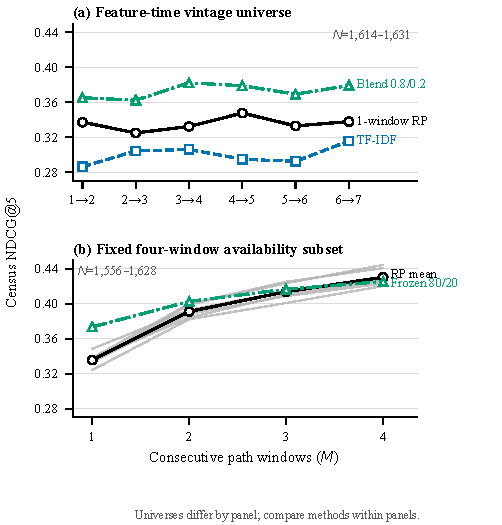
\includegraphics[width=0.94\columnwidth]{figures/fig_acceptance_robustness.pdf}
\caption{Modern walk-forward NDCG@5.  \textbf{(a)}~One-period path, TF-IDF,
and frozen blend.  \textbf{(b)}~Path and the same blend by memory length on a
fixed availability subset; thin lines are transitions and heavy lines are
means.  Fusion helps at $M=1,2$, but not $M=4$.  Panels use different universes.}
\Description{Panel a shows the frozen return-text blend above each standalone
method. Panel b shows return-path and frozen-blend means converging as return
history grows, with the return path above fusion at four periods.}
\label{fig:acceptance_robustness}
\end{figure}

\begin{table}[t]
\caption{Six-transition walk-forward NDCG@5 (all queries; mean $\pm$
descriptive population SD).  Groups use different eligibility rules.
$\ddagger$~Transductive; spectral cosine is within $0.002$ and omitted.}
\label{tab:results}
\small\setlength{\tabcolsep}{4pt}
\begin{tabular}{llc}
\toprule
\textbf{Universe} & \textbf{Method} & \textbf{WF NDCG@5} \\
\midrule
Full return & Return path & $\mathbf{0.339\pm0.007}$ \\
            & Spectral dot (rank\,128)$^\ddagger$ & $0.336\pm0.006$ \\
            & SIC-2 & $0.213\pm0.009$ \\
            & Random & $0.118\pm0.006$ \\
\midrule
Vintage 10-K & Frozen rank blend (80/20) & $\mathbf{0.373\pm0.008}$ \\
             & Return path & $0.336\pm0.007$ \\
             & Vintage TF-IDF & $0.300\pm0.010$ \\
             & Granite-r2 (stored excerpt) & $0.279\pm0.006$ \\
             & Granite-r2 (512 tok.) & $0.259\pm0.006$ \\
             & Vintage SEC-BERT & $0.256\pm0.009$ \\
             & Vintage BGE & $0.256\pm0.007$ \\
             & Vintage MiniLM & $0.215\pm0.006$ \\
\midrule
Four-period history & Concatenated return path & $\mathbf{0.430\pm0.009}$ \\
\bottomrule
\end{tabular}
\end{table}

\subsection{Regime Robustness and Historical Extension}
\label{sec:temporal}

We next test whether the return path's advantage over standalone text methods
extends across market regimes and the earlier 2020--2024 period.

We construct 13 additional non-overlapping calendar blocks (H1--H13; $T = 62$--$86$
trading days each, or approximately three to four months) spanning
February~2020--April~2024, adjacent to W1 on the next-trading-day boundary.
These periods contain $N=1{,}389$--$1{,}666$ firms with complete returns and
$1{,}264$--$1{,}547$ with vintage text.  Vintage 10-K coverage among firms with
complete feature-period returns is
$89.5$--$93.8\%$ historically versus $82.3$--$84.1\%$ in W1--W6, and
the historical periods contain $T=62$--$86$ trading days.  The resulting mean
($0.364$) is therefore not directly comparable to
Table~\ref{tab:results} ($0.336$).
NDCG@5 is higher in the high-volatility tercile.  Because the regimes are
descriptive and NDCG is normalized within query, we compare methods within
transitions and do not interpret NDCG levels across periods.
H13 ends the day preceding W1; the same FF5 residual, LW shrinkage, metric, and
feature-time text rule are applied throughout.
The extension spans the COVID-19 crash and the 2022 rate shock.
TF-IDF weights are fitted per window.
Each transition is labeled by the annualized volatility, during $W_t$, of the
Fama--French market excess-return factor (Mkt-RF).  The 33rd and 67th percentiles
across all 20 windows label 7 high-, 6 medium-, and 6 low-volatility
transitions.  Because these thresholds use the full panel, the labels are
descriptive rather than an ex-ante classifier.
The return path leads in all three regimes (Table~\ref{tab:historical}).  We
emphasize the observed within-transition ordering and treat the win counts
descriptively.
As a dependence check, odd- and even-indexed sets avoid direct reuse of adjacent
periods.  The return path wins 9/10 in the odd set and 9/9 in the even set.
Securities and regimes remain shared, so the counts are not independent trials.
Only H1$\to$H2 reverses the ordering (TF-IDF leads by $0.039$;
Fig.~\ref{fig:regime_timeline}); one transition cannot establish whether the
crash-to-recovery change explains it.

\begin{table}[t]
\caption{Walk-forward NDCG@5 by volatility regime over 19 transitions spanning
2020--2026 (mean $\pm$ population SD; all queries per transition; LW shrinkage
$\delta\in[0.62,0.81]$ across the full 20-window panel).
TF-IDF vocabulary and IDF weights are fitted separately on each window's
corpus.}
\label{tab:historical}
\small
\begin{tabular}{lcc}
\toprule
\textbf{Regime} & \textbf{Return path} & \textbf{TF-IDF} \\
\midrule
All (19 trans.) & $0.364\pm0.033$ & $0.318\pm0.022$ \\
High-vol (7)    & $0.381\pm0.038$ & $0.333\pm0.019$ \\
Medium-vol (6)  & $0.358\pm0.030$ & $0.317\pm0.022$ \\
Low-vol (6)     & $0.348\pm0.017$ & $0.302\pm0.012$ \\
\midrule
\multicolumn{1}{l}{Return path wins} & \multicolumn{2}{c}{18/19} \\
\bottomrule
\end{tabular}
\end{table}

\begin{figure}[t]
\centering
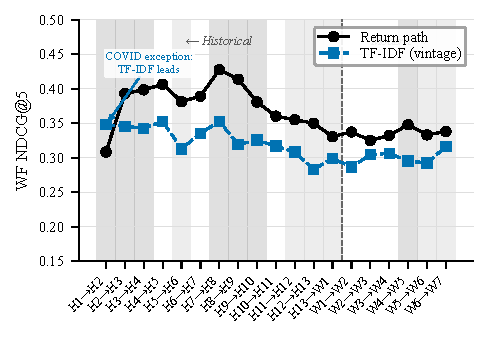
\includegraphics[width=0.90\columnwidth]{figures/fig_regime_timeline.pdf}
\caption{WF NDCG@5 per transition across the full 20-window, 19-transition evaluation
(2020--2026; vintage-correct 10-K text; \S\ref{sec:temporal}).
Shading: high-volatility (darker), low-volatility (lighter), medium unshaded.
Dashed line separates the historical extension (left) from W1--W7 (right).
The return path leads in 18 of 19 transitions.}
\Description{Line chart over 19 transitions. The return path is highest in 18, TF-IDF in 1.
Regime shading shows the advantage persists across volatility terciles.}
\label{fig:regime_timeline}
\end{figure}

\subsection{Robustness Checks}
\label{sec:robustness}

\textbf{Ticker-syntax exclusion.}
A rule based on vendor ticker suffixes flags the same 118 possible preferred or
non-primary share classes among firms eligible at each modern ranking date.
After excluding them and refitting TF-IDF ($N=1{,}496$--$1{,}513$), the return
path remains ahead in 6/6 transitions: $0.324\pm0.007$ versus
$0.301\pm0.011$, a gap of $0.023$.  Relative to the unrestricted universe, their mean changes
are $-0.012$ and $+0.001$, respectively.  The ticker rule is only a syntax check
and does not identify common stocks authoritatively.

\textbf{Residual-magnitude audit.}
Daily adjusted-price FF5 residuals include a few extreme magnitudes.  Excluding
any security whose maximum absolute raw residual exceeds 1.0 in decimal-return
units (100 percentage points) in either the feature or target period removes
148 of 9{,}723 transition--security rows
(1.52\%; $N=1{,}587$--$1{,}604$); after refitting TF-IDF and fully reranking,
NDCG@5 is $0.340/0.305/0.378$ for return path/TF-IDF/blend.  A stricter threshold
of 0.5 (50 percentage points) and feature-period screens at thresholds of 1.0
and 0.5 retain both method orderings in 6/6 transitions.  Because screens that
use either period inspect $W_{t+1}$ and a large
residual may be genuine, we use them only as retrospective data-quality checks.

\textbf{Depth, weighting, and coverage.}
The return path exceeds TF-IDF at every tested depth
$k\in\{1,5,10,20\}$ (respective macro means
$0.356/0.336/0.329/0.326$ versus $0.317/0.300/0.288/0.280$), and in 6/6
transitions at each depth.  Giving recent days more weight with a fixed,
RiskMetrics-style exponentially weighted moving average (EWMA) does not help:
paths with 20- and 40-day half-lives
attain $0.321$ and $0.331$, versus $0.336$
unweighted.
Requiring 10-K coverage only in $W_t$ adds 0--3 names relative to requiring it
in both $W_t$ and $W_{t+1}$, and changes both return-path and TF-IDF means by
less than $0.001$.

\textbf{Sensitivity to target dates.}
With rankings fixed, 1{,}000 circular block resamples per target period jointly
resample contiguous 5- or 10-day blocks across all securities.  The empirical
2.5th--97.5th percentiles give conditional 95\% ranges of
$[0.031,0.038]$ for return path minus TF-IDF and $[0.029,0.036]$ for blend
minus return path.  All six gaps remain positive in every replicate.  The ranges
describe conditional sensitivity and should not be read as confidence intervals.

\textbf{Encoder context length.}
The median stored vintage Item~1 excerpt reaches the 8,000-character
collection cap (85.9\% reach it) and contains 1,511 Granite tokens;
94.6\% exceed 512, while none exceed 8,192.  Encoding the full stored excerpts
raises Granite from $0.259\pm0.006$ at 512 tokens to $0.279\pm0.006$ and improves
its score in all six transitions.  Granite still trails TF-IDF and the return
path in every transition.  The test covers the stored excerpts, which may still
truncate Item~1.

\textbf{Historically trained nonlinear fusion.}
A histogram-based gradient-boosted pairwise ranker trained on twelve 2020--2024
transitions from return/text ranks and similarities, then frozen, attains
$0.308\pm0.009$ and trails both the one-window path and fixed rank blend in
6/6 modern transitions.  We include this model as a supervised diagnostic; the
experiment does not cover the full range of learned peer models.

% v1 negative result: run_20260802_v1, historical_selection.json
A second diagnostic replaces the fixed blend with a gated two-tower encoder: a
temporal convolutional neural network (CNN) over residual paths, a frozen text
projection, and a direct path for raw-return inputs.  Trained and selected only
on the same twelve historical transitions under a pre-registered continuation
rule, it fails decisively:
mean NDCG@5 is $0.377$ versus $0.409$ for the frozen blend across the six
continuation tests, with 0/6 wins and little variation across seeds.  As
required, the model never accesses modern-transition targets.
Neither trained model displaces the simple frozen blend under historical-only
selection, supporting the residual path as a required baseline.

\textbf{Contemporaneous text performance.}
Using the same eligible firms and frozen representations in each transition as
the primary walk-forward comparison, but evaluating against
$W_t$ rather than $W_{t+1}$ correlations, same-window NDCG@5 is
$0.297\pm0.007$ for TF-IDF, $0.257\pm0.006$ for 512-token Granite-r2, and
$0.213\pm0.004$ for MiniLM.  The corresponding walk-forward values are
$0.300\pm0.010$, $0.259\pm0.006$, and $0.215\pm0.006$; the largest unrounded
gap is $0.0035$.  Within this diagnostic, contemporaneous evaluation does not
close the text--return gap.  Return availability in
$W_{t+1}$ is retained only to match the primary comparison universe.

\paragraph{Reproducibility.}
The paper is self-contained; code, window scripts, and hashed results are
archived for release after review.  Packages are pinned
(\texttt{requirements.lock}); seeds, tie-breaking, and window parameters appear
in Table~\ref{tab:config}.
Price data come from Yahoo Finance via \texttt{yfinance}.  Encoder weights are frozen public
checkpoints.  Raw price panels and per-security residual arrays are not
redistributed; exact regeneration depends on Yahoo's adjusted history, which
may be revised after acquisition.  Frozen result files and their hashes are the
authoritative numerical record.

% ══════════════════════════════════════════════════════════════════════
\section{Discussion}
\label{sec:discussion}

\begin{table}[t]
\caption{Audit of lists fixed at ranking time (six equally weighted
transitions).  Lists are fixed before target returns; incomplete query--list
pairs are dropped without reranking.  For each list, $r_{qB}$ correlates the query's raw
$W_{t+1}$ FF5 residual path with the daily equal-weight mean of its five peer
paths; $\overline r_{qB}$ is its mean.  Pos.
is the share with $r_{qB}>0$, and Eval. is the share with observed target
returns, conditional on $W_t$ return and vintage-text eligibility
($N=1{,}615$--$1{,}632$).  Positivity is directional, not a
significance or economic-utility threshold.}
\label{tab:application}
\small\setlength{\tabcolsep}{4pt}
\begin{tabular}{lccc}
\toprule
\textbf{Retrieval} & $\overline r_{qB}$ & \textbf{Pos.} & \textbf{Eval.} \\
\midrule
Return path & 0.208 & 74.1\% & 99.2\% \\
TF-IDF & 0.186 & 77.9\% & 99.4\% \\
Frozen blend & \textbf{0.248} & \textbf{79.7\%} & 99.6\% \\
SIC-2 & 0.118 & 71.6\% & 99.5\% \\
Random & 0.007 & 50.9\% & 99.4\% \\
\bottomrule
\end{tabular}
\end{table}

\paragraph{Return-path interpretation.}
The return path directly encodes sample correlation in one period.  Its
empirical value comes from how well the resulting neighbor ranking persists
into the next period.

\paragraph{What the modalities capture.}
Filing text and residual returns encode different objects.  Text primarily
describes products and operations.  Residual co-movement can reflect shared
shocks, ownership, supply chains, or return drivers omitted from FF5
~\citep{barberis2005comovement,cohen2008economic,anton2014connected}.
The comparison asks whether semantic similarity can recover this pattern when
recent residual-return observations are available.  The path is the stronger
standalone signal.  Combining text and returns helps with one or two periods of
return history, but not four.  Filing text without return history remains
untested.

\paragraph{Pairwise alignment.}
Among firms eligible when the W1 ranking is formed ($N=1{,}614$; 1{,}301{,}691
unordered pairs), Spearman correlation for the four dense encoders is only
$0.029$--$0.046$ against W1 residual correlation and $0.027$--$0.049$ against
W2.  TF-IDF is $0.036/0.035$, versus $1.000/0.103$ for the return path
(W1/W2).  These finite-panel coefficients are descriptive because pairs share
securities and target-return observations.  They summarize global pairwise
ordering, whereas NDCG@5 evaluates only five candidates per query.

\paragraph{Practical use.}
The motivating screen is refreshed only after the period's adjusted prices and
public FF5 factors are available.  An analyst would inspect its five candidates
together with industry or valuation peers.  The index stores 47--77 float32
values per security and requires a complete aligned path.  For a new company or
one with little history, a production system must abstain or use an
untested fallback.  Liquidity, stock-borrow availability, costs, and position
constraints do not enter ranking.  Production latency, factor-publication lag,
data revisions, and analyst adoption are not measured here.

% ══════════════════════════════════════════════════════════════════════
\section{Limitations}
\label{sec:limitations}

\paragraph{Data and universe.}
The retrospectively assembled 2{,}200-ticker panel is not a point-in-time
security master, so the historical extension is conditioned on later survival
and news visibility.  This may favor firms with stable exposures, but we cannot
determine the direction of the resulting bias.
Requiring complete returns in each period further favors liquid, surviving names; share classes
and non-primary securities are not comprehensively removed.  A ticker-syntax
audit flags 118 possible preferred or non-primary names in the modern
evaluation.  The flag is not a definitive security classification.  Results
apply to this panel and should not be generalized to all U.S.\ common stocks.
Non-U.S.\ markets are untested.  Yahoo histories lack Center for Research in Security Prices
(CRSP)-style delisting returns, security
typing, and verified corporate-action adjustments.  Residual-magnitude screens
serve only as sensitivity checks and are not error labels.

\paragraph{Information sets and statistical scope.}
Because recent returns closely match the information needed to estimate future
co-movement, the return representation has a deliberate advantage.  The
experiment tests whether that advantage persists; it cannot establish that the representation
is optimal for other peer definitions.  The primary modern NDCG evaluation defines
its evaluated universe using complete returns in $W_t$ and $W_{t+1}$.  This
makes it a retrospective benchmark, not a live backtest.  A separate audit
fixes rankings among firms eligible at $W_t$, then reports attrition without reranking
(99.2--99.6\% target evaluability).  The rate is conditional on firms having
returns and vintage text at ranking time.  That selection universe
covers 82.3--84.1\% of the complete-return universe, not deployment coverage.
The candidate set is still retrospective, so this is not a backtest built from
a point-in-time security master.
Adjacent transitions share one period, and queries share dates, candidates, and
target matrices.  These dependencies rule out IID inference.  We report panel
means, transition standard deviations, and win counts descriptively.  Resampling target dates preserves
common shocks but remains conditional on the observed regimes and does not
establish population or cross-regime uncertainty.

\paragraph{Model and metric scope.}
The return path is unavailable for a newly listed security with no return
history (a cold start) and otherwise requires a complete shared history.  The
experiments use one family of roughly quarterly windows, positive-correlation
relevance, U.S.\ data, and no transaction-cost or portfolio optimization
objective.  NDCG is relative to each query's attainable ranking.  Five names
represent an illustrative analyst workload.  We do not validate a minimum-correlation
threshold, abstention rule, or utility--coverage
curve relating performance to the share of queries served.
Retrieval depth is tested at $k=1,5,10,20$, but
temporal weighting is limited to two fixed half-lives and a descriptive
concatenation of one to four periods.
FF5-residual correlation is one peer definition among several.  It does not
reward same-issuer relationships that a valuation- or disclosure-based
definition would rank first.  Filing comparators are frozen off-the-shelf
encoders.  Because 85.9\% of excerpts hit the 8,000-character collection cap,
even the full-excerpt Granite run does not cover the complete section.  MiniLM, BGE, and
SEC-BERT use 128--512-token inputs (\S\ref{sec:robustness}).  Other current
retrieval encoders, supervised filing models, risk factors (Item~1A),
Management's Discussion and Analysis (MD\&A), news, and Form~S-1 registration filings,
and vintage-aligned
TNIC~\citep{hoberg2016text} remain open comparisons.

% ══════════════════════════════════════════════════════════════════════
\section{Conclusion}
\label{sec:conclusion}

Semantic filing similarity is not a proxy for behavioral similarity in this
experiment.  Across 1,301,691 pairs, four dense encoders have Spearman
correlations of only $0.029$--$0.046$ with same-quarter residual co-movement and
$0.027$--$0.049$ with next-quarter co-movement.  Semantically similar firms, in
other words, need not be behavioral peers.  Yet text still helps at the top of
the ranking when return history is short: the return path reaches NDCG@5
$0.336\pm0.007$ and leads every standalone filing comparator, while a
return--text blend reaches $0.373\pm0.008$ and improves all six modern
transitions.  Across 19 transitions the path leads TF-IDF in 18.  The gain from
text disappears with four periods of return history.

A separate audit freezes lists before target returns, leaves missing candidates
unreplaced, and retains the blend's aggregate lead.  It measures co-movement and
evaluability, not exposure discovery, risk reduction, or analyst decisions.

For this return-defined task, recent return paths are a short, interpretable
baseline when history exists.  Other information settings require different
encodings.

\paragraph{Generative-AI disclosure.}
OpenAI Codex and Anthropic Claude Code assisted with design review, writing,
code refactoring, and result checks.  The authors reviewed all text and code,
reran the experiments, verified citations and numerical claims, and take
responsibility for the work.

% ══════════════════════════════════════════════════════════════════════
\bibliographystyle{ACM-Reference-Format}
\bibliography{references}

\end{document}
